\documentclass[12pt]{article}
\usepackage[letterpaper, total={6in, 8in}]{geometry}
\setlength{\oddsidemargin}{0in}
\setlength{\evensidemargin}{0in}
\setlength{\textwidth}{6.5in}
\setlength{\parindent}{0in}
\setlength{\parskip}{\baselineskip}

\usepackage{amsmath,amsfonts,amssymb}
\usepackage{subfigure}
\usepackage{sectsty}
\usepackage{multirow}
\usepackage{makecell}
\usepackage{float}
\usepackage[utf8x]{inputenc}
\usepackage[pdftex]{graphicx}
\usepackage[toc,page]{appendix}
\usepackage{enumitem}
\usepackage{indentfirst}
\usepackage{scrextend}
\usepackage{caption}
\usepackage{hyperref}
\usepackage{adjustbox}

\usepackage{listings}
\usepackage{color} %red, green, blue, yellow, cyan, magenta, black, white
\definecolor{mygreen}{RGB}{28,172,0} % color values Red, Green, Blue
\definecolor{mylilas}{RGB}{170,55,241}

\DeclareFixedFont{\ttb}{T1}{txtt}{bx}{n}{10} % for bold
\DeclareFixedFont{\ttm}{T1}{txtt}{m}{n}{10}  % for normal

\usepackage{color}
\definecolor{deepblue}{rgb}{0,0,0.5}
\definecolor{deepred}{rgb}{0.6,0,0}
\definecolor{deepgreen}{rgb}{0,0.5,0}

\usepackage{sectsty}

\sectionfont{\fontsize{14}{15}\selectfont}
\subsectionfont{\fontsize{12}{15}\selectfont}

\usepackage{listings}
\lstset{language=Matlab,%
	%basicstyle=\color{red},
	breaklines=true,%
	morekeywords={matlab2tikz},
	keywordstyle=\color{blue},%
	morekeywords=[2]{1}, keywordstyle=[2]{\color{black}},
	identifierstyle=\color{black},%
	stringstyle=\color{mylilas},
	commentstyle=\color{mygreen},%
	showstringspaces=false,%without this there will be a symbol in the places where there is a space
	numbers=left,%
	numberstyle={\tiny \color{black}},% size of the numbers
	numbersep=9pt, % this defines how far the numbers are from the text
	emph=[1]{for,end,break},emphstyle=[1]\color{red}, %some words to emphasise
	%emph=[2]{word1,word2}, emphstyle=[2]{style},    
}


% Python style for highlighting
\newcommand\pythonstyle{\lstset{
		language=Python,
		basicstyle=\ttm,
		otherkeywords={self},             % Add keywords here
		keywordstyle=\ttb\color{deepblue},
		emph={MyClass,__init__},          % Custom highlighting
		emphstyle=\ttb\color{deepred},    % Custom highlighting style
		stringstyle=\color{deepgreen},
		frame=tb,                         % Any extra options here
		showstringspaces=false            % 
}}


% Python environment
\lstnewenvironment{python}[1][]
{
	\pythonstyle
	\lstset{#1}
}
{}

% Python for external files
\newcommand\pythonexternal[2][]{{
		\pythonstyle
		\lstinputlisting[#1]{#2}}}

% Python for inline
\newcommand\pythoninline[1]{{\pythonstyle\lstinline!#1!}}

\begin{document}
\hfill Sam Feig $|$ Vladimir Zhdanov \\
\textbf{H5 Report}\hfill CSCI 4831/5722 \\
\rule{\textwidth}{.75pt}

\section{Methods}

\subsection{Computing Feature Vectors}
\subsection{Feature Normalization}

\section{Visualizations}

\subsection{Successful Segmentations}
\begin{figure}[H]
	\centering
	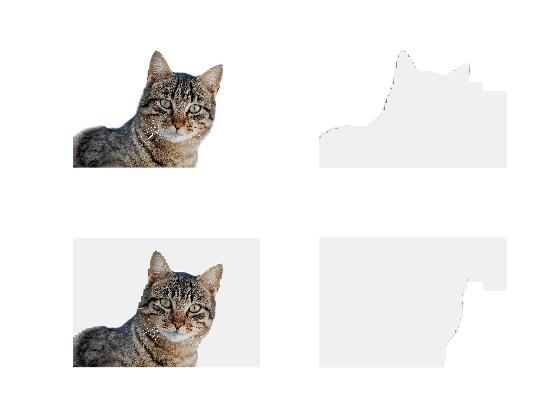
\includegraphics[width=.9\textwidth]{succ1.jpg}
	\caption{\texttt{cat\_march.jpg}, using HAC with $k = 3$, position + color features, feature normalization, and a resize factor of $0.025$.}
\end{figure}

\begin{figure}[H]
	\centering
	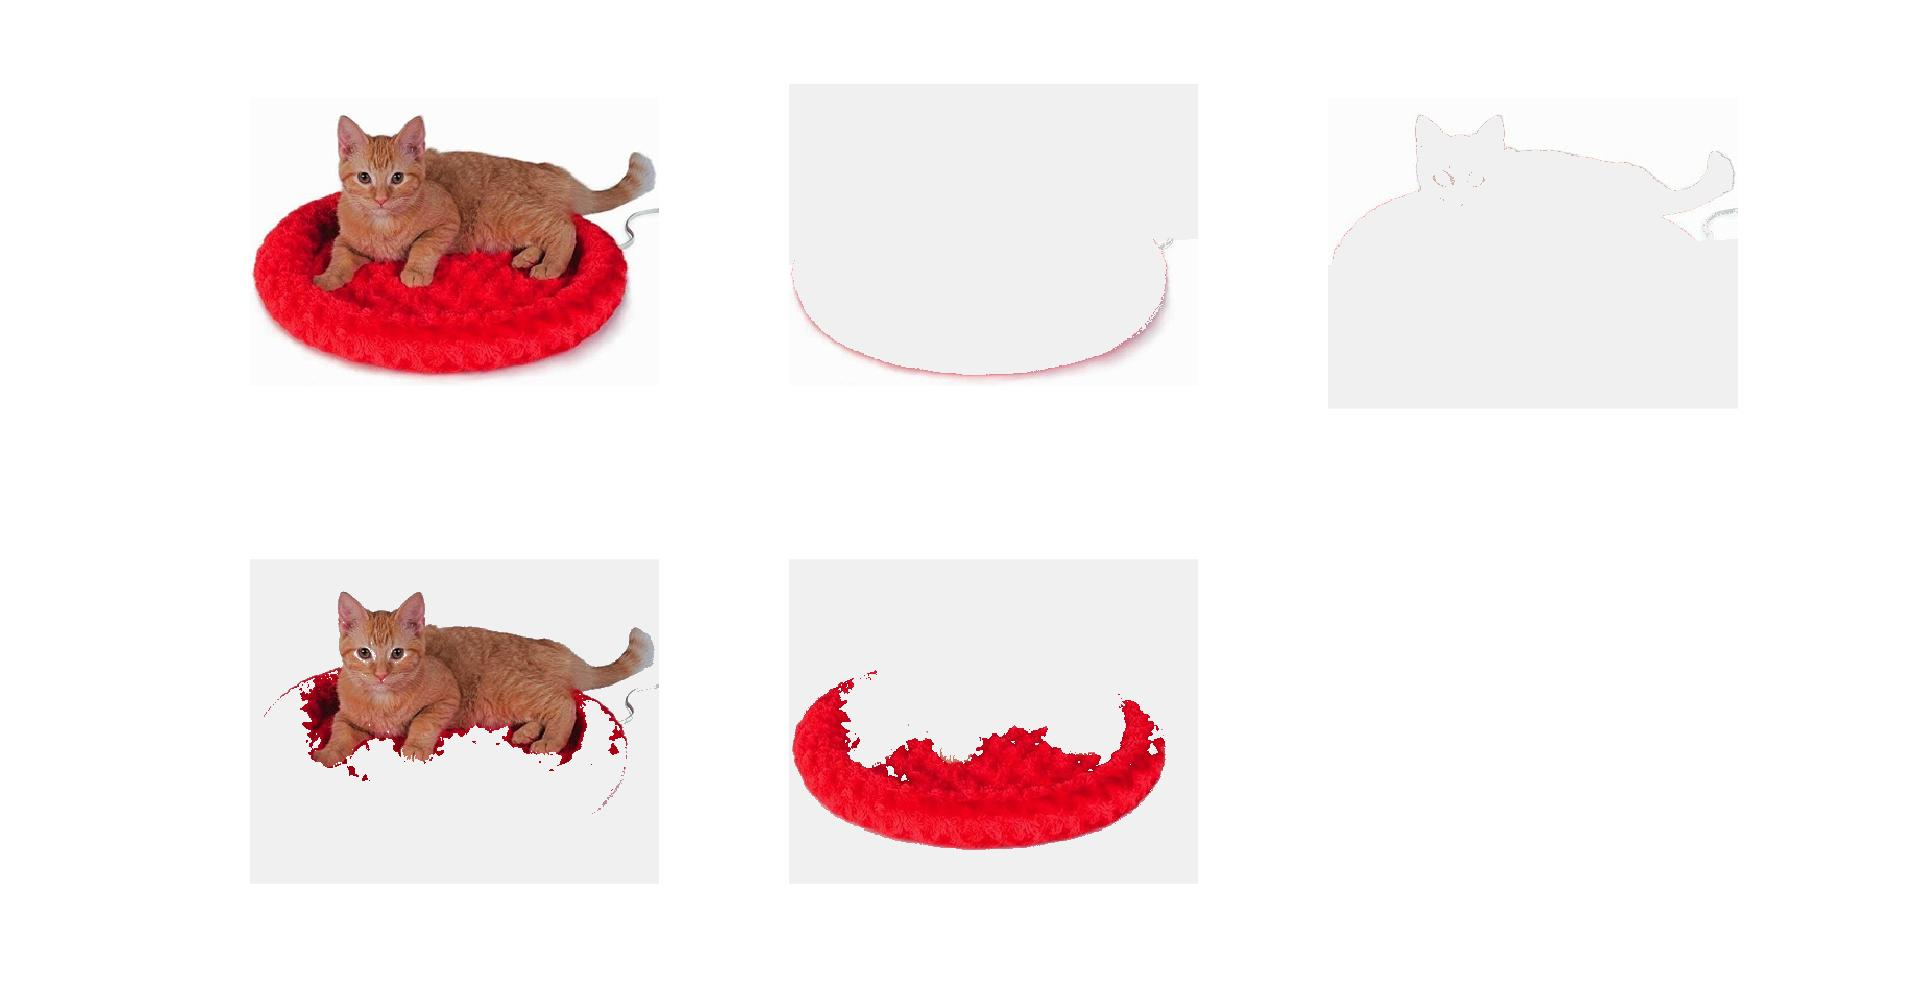
\includegraphics[width=.95\textwidth]{succ2.jpg}
	\caption{\texttt{Cat\_Bed.jpg}, using k-means clustering with $k = 4$, position + color features, and feature normalization.}
\end{figure}

\begin{figure}[H]
	\centering
	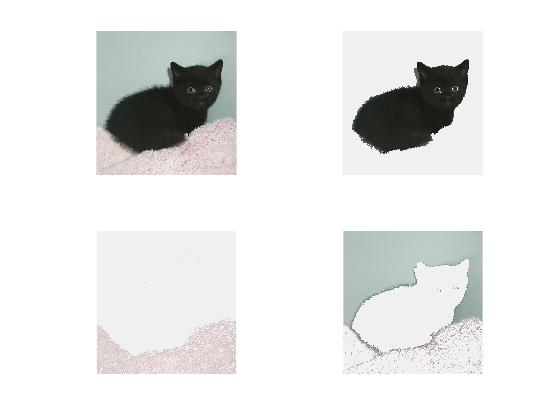
\includegraphics[width=.95\textwidth]{succ3.jpg}
	\caption{\texttt{black\_kitten\_star.jpg}, using k-means clustering with $k = 3$, color features, and no feature normalization.}
\end{figure}

\subsection{Unsuccessful Segmentations}
\begin{figure}[H]
	\centering
	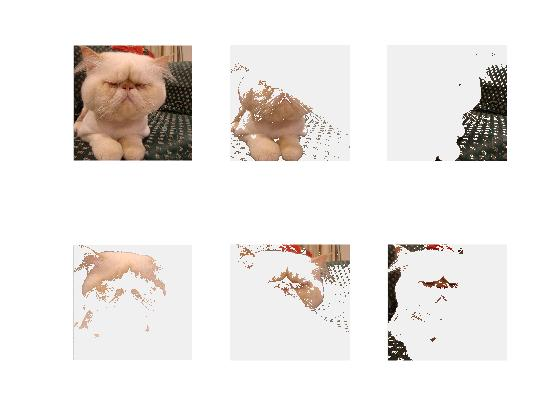
\includegraphics[width=.9\textwidth]{unsucc1.jpg}
	\caption{\texttt{cat\_grumpy.jpg}, using k-means clustering with $k = 5$, position + color features, and no feature normalization.}
\end{figure}

\begin{figure}[H]
	\centering
	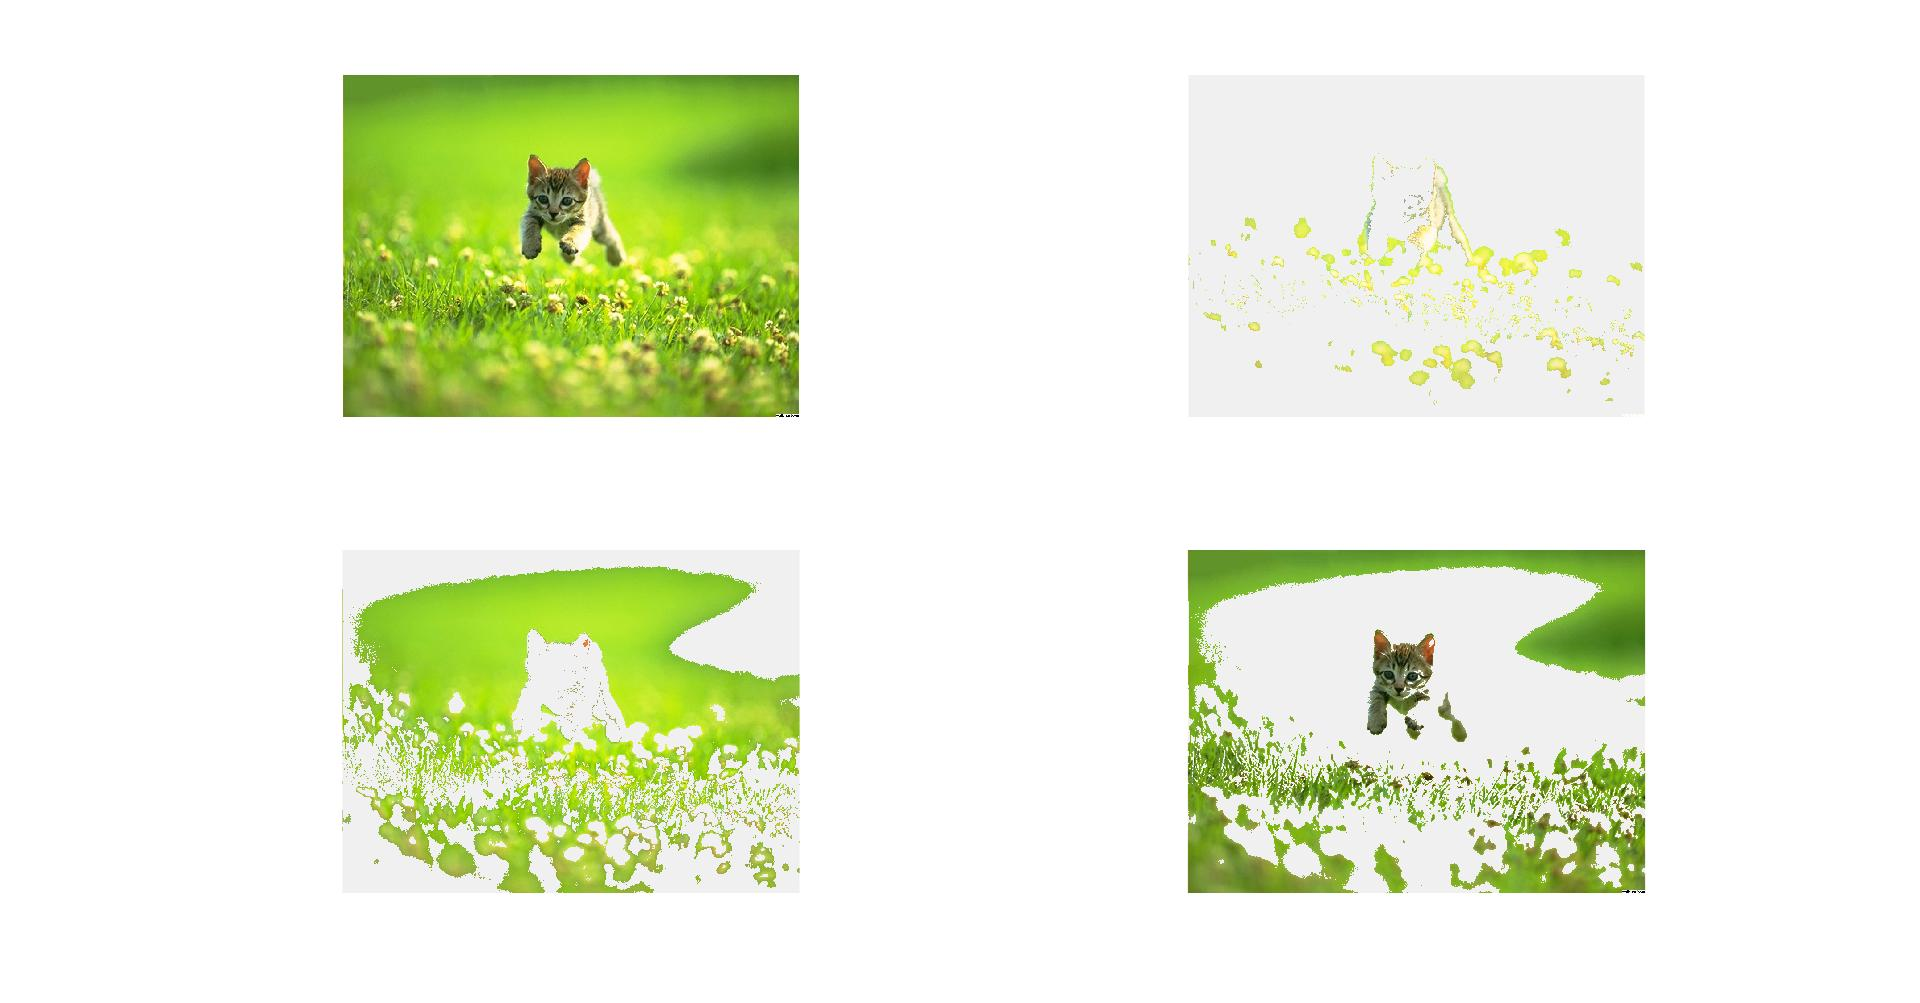
\includegraphics[width=.95\textwidth]{unsucc2.jpg}
	\caption{\texttt{cat-jumping-running-grass.jpg}, using k-means clustering with $k = 3$, color features, and feature normalization.}
\end{figure}

\begin{figure}[H]
	\centering
	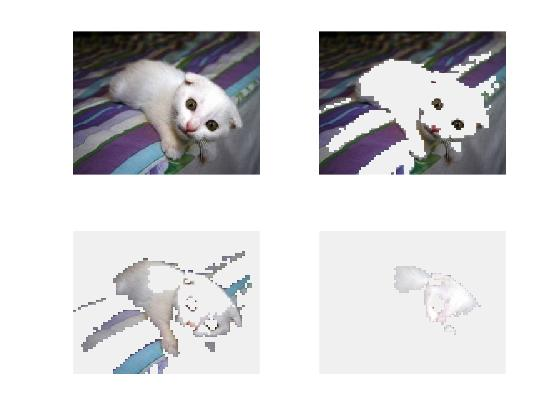
\includegraphics[width=.95\textwidth]{unsucc3.jpg}
	\caption{\texttt{kitten16.jpg}, using HAC with $k = 3$, color features, feature normalization, and a resize factor of $0.25$.}
\end{figure}

\subsection{Composite Images}
Using the script titled \texttt{GrabCat.m}, we were able to produce composite images by transferring segments from one image to another background image. This allowed us to create the two composite images shown below.

\begin{figure}[H]
	\centering
	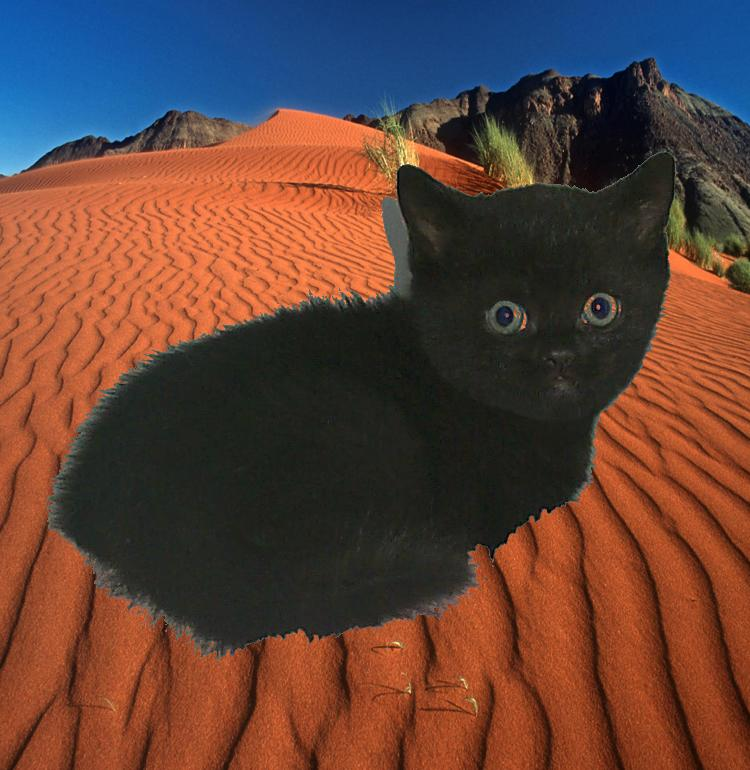
\includegraphics[width=.5\textwidth]{grabcat1.jpg}
	\caption{Input: \texttt{black\_kitten\_star.jpg, desert.jpg}, using k-means clustering with $k = 3$, color features, and feature normalization.}
\end{figure}

\begin{figure}[H]
	\centering
	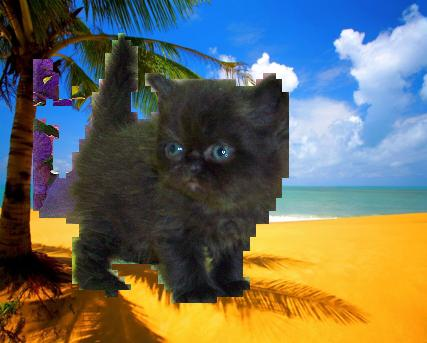
\includegraphics[width=.5\textwidth]{grabcat2.jpg}
	\caption{Input: \texttt{black\_kitten.jpg, beach.jpg}, using HAC with $k = 5$, color features, feature normalization, and a resize factor of $0.2$.}
\end{figure}

\section{Evaluation}

\begin{table}[H]
	\begin{adjustbox}{width=\columnwidth,center}
		\begin{tabular}{c c c c c c}
			\hline
			\textbf{Feature} & \textbf{Feature} & \textbf{Clustering} & \textbf{Number} & \textbf{Resize} & \textbf{Mean} \\
			\textbf{Transform} & \textbf{Normalization} & \textbf{Method} & \textbf{of Clusters} & \textbf{(Max Pixels)} & \textbf{Accuracy} \\
			\hline
			Color & Yes & K-Means & 3 & 50000 & .8341 \\
			Color & Yes & K-Means & 5 & 50000 & .8736 \\
			Color & Yes & K-Means & 7 & 50000 & .8795 \\
			Color & Yes & K-Means & 15 & 50000 & .9087 \\
			Color & Yes & K-Means & 30 & 50000 & .9228 \\
			Color & No  & K-Means & 5 & 50000 & .8680 \\
			Color/Position & Yes & K-Means & 5 & 50000 & .8765 \\
			Color/Position & No & K-Means & 5 & 50000 & .8802 \\
			Color/Edges & Yes & K-Means & 5 & 50000 & .7991\\
			Color/Edges & No & K-Means & 5 & 50000 & .8670 \\
			Color/Gradients & Yes & K-Means & 5 & 50000 & .7905 \\
			Color/Gradients & No & K-Means & 5 & 50000 & .8775 \\
			Color/Position/Edges & Yes & K-Means & 5 & 50000 & .7951 \\
			Color/Position/Edges & No & K-Means & 5 & 50000 & .8800 \\
			Color/Position/Edges/Gradients & Yes & K-Means & 5 & 50000 & .7924 \\
			Color/Position/Edges/Gradients & No & K-Means & 5 & 50000 & .8866 \\
			Color & Yes & HAC & 5 & 1000 & .8623 \\
			Color & Yes & HAC & 3 & 1000 & .8340 \\
			Color & Yes & HAC & 7 & 1000 & .8691 \\
			Color & Yes & HAC & 15 & 1000 & .8906 \\
			Color & Yes & HAC & 15 & 1000 & .9123 \\
			Color & No & HAC & 5 & 1000 & .8585 \\
			Color/Position & Yes & HAC & 5 & 1000 & .8531 \\
			Color/Position & No & HAC & 5 & 1000 & .8585 \\
			Color/Edges & Yes & HAC & 5 & 1000 & .9288 \\
			Color/Edges & No & HAC & 5 & 1000 & .8585 \\
			Color/Gradients & Yes & HAC & 5 & 1000 & .9108 \\
			Color/Gradients & No & HAC & 5 & 1000 & .8578 \\
			Color/Position/Edges & Yes & HAC & 5 & 1000 & .9256 \\
			Color/Position/Edges & No & HAC & 5 & 1000 & .8585 	\\
			Color/Position/Edges/Gradients & Yes & HAC & 5 & 1000 & .9052 \\
			Color/Position/Edges/Gradients & No & HAC & 5 & 1000 & .8550 \\
			Color & Yes & K-Means & 5 & 1000 & .8610 \\
			Color & Yes & K-Means & 5 & 10000 & .8649 \\
			Color & Yes & K-Means & 5 & 100000 & .8666 \\
			Color & Yes & HAC & 5 & 2000 & .8638 \\
			Color & Yes & HAC & 5 & 4000 & .8702 \\
		\end{tabular}
	\end{adjustbox}
\end{table}

\end{document}

